\documentclass[12pt,a4paper]{article}

% 导入必要的宏包
\usepackage[UTF8]{ctex}
\usepackage{geometry}
\usepackage{amsmath}
\usepackage{amsfonts}
\usepackage{amssymb}
\usepackage{graphicx}
\usepackage{enumitem}
\usepackage{xcolor}
\usepackage{tikz}
\usepackage{float}
\usepackage{hyperref}
\usepackage{multicol}
\usepackage{longtable}
\usepackage{array}
\usepackage{tabularx}

% 页面设置
\geometry{left=2.5cm,right=2.5cm,top=2.5cm,bottom=2.5cm}

% 标题页设置
\title{\textbf{2016年数据结构题库} \\ \large 单项选择题与综合应用题详解}
\author{}
\date{}

% 定义题型环境
\newenvironment{choicequestion}[1][]{%
    \vspace{0.5cm}
    \noindent\textbf{[#1]}
    \vspace{0.2cm}
}{}

\newenvironment{answersection}{%
    \vspace{0.2cm}
    \noindent\textbf{[参考答案]}\\
    \vspace{0.1cm}
}{}

\newenvironment{analysissection}{%
    \vspace{0.2cm}
    \noindent\textbf{[答案解析]}\\
    \vspace{0.1cm}
}{}

% 定义题号计数器
\newcounter{questioncounter}

% 定义题号计数器
\newcounter{questioncounter}

% 问题格式化命令
\newcommand{\question}[2]{%
    \stepcounter{questioncounter}%
    \noindent\textbf{\thequestioncounter} #1%
}

% 选择题选项格式
\newcommand{\choices}[4]{%
    \begin{multicols}
    \noindent \textbf{A.} #1 \par
    \noindent \textbf{B.} #2 \par
    \noindent \textbf{C.} #3 \par
    \noindent \textbf{D.} #4 \par
    \end{multicols}%
}

% 开始文档
\begin{document}

\maketitle

\section{单项选择题}

\begin{choicequestion}[单选题]
\question{已知表头元素为 c 的单链表在内存中的存储状态如下表所示。\newline

\begin{table}[h]
\centering
\begin{tabular}{|c|c|c|}
\hline
地址 & 元素 & 链接地址 \\
\hline
1000H & a & 1010H \\
\hline
1004H & b & 100CH \\
\hline
1008H & c & 1000H \\
\hline
100CH & d & NULL \\
\hline
1010H & e & 1004H \\
\hline
1014H & & \\
\hline
\end{tabular}
\end{table}\newline

现将f存放于1014H处并插入到单链表中，若f在逻辑上位于a和e之间，则a,e,f的"链接地址"依次是}{}

\choices{$1010\mathrm{H}, 1014\mathrm{H}, 1004\mathrm{H}$}{$1010\mathrm{H}, 1004\mathrm{H}, 1014\mathrm{H}$}{$1014\mathrm{H}, 1010\mathrm{H}, 1004\mathrm{H}$}{$1014\mathrm{H}, 1004\mathrm{H}, 1010\mathrm{H}$}

\begin{answersection}
D. $1014\mathrm{H}, 1004\mathrm{H}, 1010\mathrm{H}$
\end{answersection}

\begin{analysissection}
原链表逻辑顺序为：c（1008H）$\to$ a（1000H）$\to$ e（1010H）$\to$ b（1004H）$\to$ d（100CH）。

将f（1014H）插入到a与e之间后，新顺序为：c $\to$ a $\to$ f $\to$ e $\to$ b $\to$ d。

- a的链接地址由原来的1010H（指向e）改为1014H（指向f）；
- f的链接地址为e原来的地址1010H；
- e的链接地址保持1004H（指向b）不变。

因此，a、e、f的链接地址依次是1014H、1004H、1010H。
\end{analysissection}
\end{choicequestion}

\begin{choicequestion}[单选题]
\question{已知一个带有表头结点的双向循环链表 L, 结点结构为 prev data next, 其中, prev 和 next 分别是指向其直接前驱和直接后继结点的指针。现要删除指针 p 所指的结点, 正确的语句序列是}{}

\choices{$p->next->prev = p->prev; p->prev->next = p->prev; free(p);$}{$p->next->prev = p->next; p->prev->next = p->next; free(p);$}{$p->next->prev = p->next; p->prev->next = p->prev; free(p);$}{$p->next->prev = p->prev; p->prev->next = p->next; free(p);$}

\begin{answersection}
D. $p->next->prev = p->prev; p->prev->next = p->next; free(p);$
\end{answersection}

\begin{analysissection}
删除双向循环链表中结点p时，需正确维护前驱和后继指针：

- p的后继结点的prev指针应指向p的前驱结点；
- p的前驱结点的next指针应指向p的后继结点。

语句D准确完成了上述调整，随后释放结点p。
\end{analysissection}
\end{choicequestion}

\begin{choicequestion}[单选题]
\question{设有下图所示的火车车轨，入口到出口之间有 $n$ 条轨道，列车的行进方向均为从左至右，列车可驶入任意一条轨道。现有编号为 $1 \sim 9$ 的9列列车，驶入的次序依次是8,4,2,5,3,9,1,6,7。若期望驶出的次序依次为 $1 \sim 9 $，则 $n$ 至少是}{}

\begin{figure}[H]
\centering
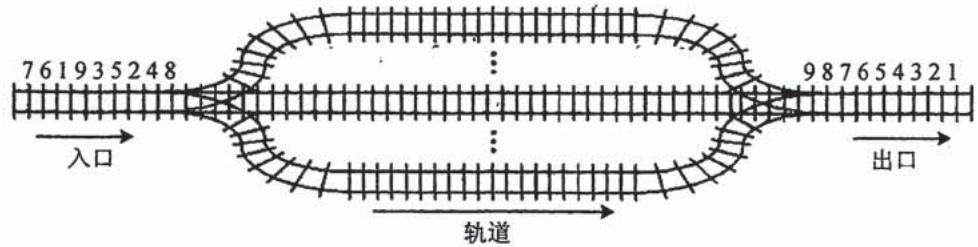
\includegraphics[width=0.4\textwidth]{images/c8b4979054462f7a389ffdaf36152317b518ecd1dd69f1dbe15bc6e5cf468b80.jpg}
\end{figure}

\choices{2}{3}{4}{5}

\begin{answersection}
C. 4
\end{answersection}

\begin{analysissection}
该问题可建模为使用多个栈（每条轨道为一个栈）对输入序列进行重排以得到目标输出序列1~9。通过模拟入轨、出轨操作可知，为保证严格的1到9递增输出顺序，在处理输入序列8,4,2,5,3,9,1,6,7时，至少需要4条轨道才能避免违背栈的后进先出特性。
\end{analysissection}
\end{choicequestion}

\begin{choicequestion}[单选题]
\question{有一个100阶的三对角矩阵 $M$ ，其元素 $m_{i,j}$ （ $1 \leqslant i \leqslant 100, 1 \leqslant j \leqslant 100$ ）按行优先依次压缩存入下标从0开始的一维数组 $N$ 中。元素 $m_{30,30}$ 在 $N$ 中的下标是}{}

\choices{86}{87}{88}{89}

\begin{answersection}
B. 87
\end{answersection}

\begin{analysissection}
三对角矩阵按行优先压缩存储规则：

- 第1行：2个元素（$m_{1,1}, m_{1,2}$）；
- 第2行至第99行：每行3个元素；
- 第100行：2个元素。

前29行的元素总数为：2 + 28×3 = 86个。

第30行中，$m_{30,29}$ 为第87个元素（下标86），$m_{30,30}$ 为第88个元素（下标87）。故$m_{30,30}$在数组N中的下标是87。
\end{analysissection}
\end{choicequestion}

\begin{choicequestion}[单选题]
\question{若森林F有15条边、25个结点，则F包含树的个数是}{}

\choices{8}{9}{10}{11}

\begin{answersection}
C. 10
\end{answersection}

\begin{analysissection}
森林中树的个数$k$满足关系：总边数 = 总结点数 - $k$。

即 $15 = 25 - k$，解得 $k = 10$。
\end{analysissection}
\end{choicequestion}

\begin{choicequestion}[单选题]
\question{下列选项中, 不是下图深度优先搜索序列的是}{}

\begin{figure}[H]
\centering
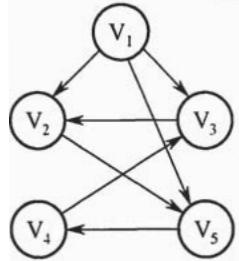
\includegraphics[width=0.3\textwidth]{images/16c1876b966f332fe0c7379c8ce523c9af595ced5e7483c50f0adbd672b3e678.jpg}
\end{figure}

\choices{$\mathrm{V}_{1}, \mathrm{V}_{5}, \mathrm{V}_{4}, \mathrm{V}_{3}, \mathrm{V}_{2}$}{$\mathrm{V}_{1}, \mathrm{V}_{3}, \mathrm{V}_{2}, \mathrm{V}_{5}, \mathrm{V}_{4}$}{$\mathrm{V}_{1}, \mathrm{V}_{2}, \mathrm{V}_{5}, \mathrm{V}_{4}, \mathrm{V}_{3}$}{$\mathrm{V}_{1}, \mathrm{V}_{2}, \mathrm{V}_{3}, \mathrm{V}_{4}, \mathrm{V}_{5}$}

\begin{answersection}
D. $\mathrm{V}_{1}, \mathrm{V}_{2}, \mathrm{V}_{3}, \mathrm{V}_{4}, \mathrm{V}_{5}$
\end{answersection}

\begin{analysissection}
深度优先搜索沿一条路径尽可能深入后再回溯。选项D呈现严格的线性连续访问顺序，与图中顶点间的实际邻接关系不符（V2与V3之间可能不存在直接边，或后续分支无法支持该访问次序）。其他三个序列均可通过不同邻接点访问顺序得到。
\end{analysissection}
\end{choicequestion}

\begin{choicequestion}[单选题]
\question{若将 $n$ （ $n > 1000$ ）个元素的升序数组 A 中查找关键字 x。查找算法的伪代码如下所示。\newline
k=0;\newline
while $(k < n$ 且 $A[k] < x)$ $k = k + 3$ ;\newline
if $(\mathbf{k} <   \mathbf{n}$ 且 $\mathrm{A}[k] == x)$ 查找成功；\newline
else if (k-1<n 且 A[k-1] == x) 查找成功;\newline
else if $(k - 2 < n$ 且 $A[k - 2] == x)$ 查找成功；\newline
else 查找失败;\newline
本算法与折半查找算法相比，有可能具有更少比较次数的情形是}{}

\choices{当 $\mathbf{x}$ 不在数组中}{当 $\mathbf{x}$ 接近数组开头处}{当 $\mathrm{x}$ 接近数组结尾处}{当 $\mathbf{x}$ 位于数组中间位置}

\begin{answersection}
C. 当 $\mathrm{x}$ 接近数组结尾处
\end{answersection}

\begin{analysissection}
该算法以步长3进行跳跃式搜索。当x接近数组结尾时，较大的跳步可快速接近目标位置，随后仅需最多3次比较即可确定结果，在此情形下比折半查找的对数级比较次数更少。
\end{analysissection}
\end{choicequestion}

\begin{choicequestion}[单选题]
\question{B+树不同于B树的特点之一是}{}

\choices{能支持顺序查找}{含有关键字}{根结点至少有两个分支}{所有叶结点都在同一层上}

\begin{answersection}
A. 能支持顺序查找
\end{answersection}

\begin{analysissection}
B+树的所有叶子结点通过指针链接成一个有序链表，从而支持高效的顺序查找和范围查询，这是B+树区别于B树的重要特征之一。
\end{analysissection}
\end{choicequestion}

\begin{choicequestion}[单选题]
\question{对 10TB 的数据文件进行排序，应使用的方法是}{}

\choices{希尔排序}{堆排序}{快速排序}{归并排序}

\begin{answersection}
D. 归并排序
\end{answersection}

\begin{analysissection}
10TB规模的数据属于外部排序问题。归并排序特别适合外部排序：可将数据分块读入内存进行内部排序，再通过多路归并逐步合并结果，高效利用磁盘I/O。
\end{analysissection}
\end{choicequestion}

\section{综合应用题}

\begin{choicequestion}[问答题]
\question{如果一棵非空 $k (k \geqslant 2)$ 叉树 $T$ 中每个非叶结点都有 $k$ 个孩子，则称 $T$ 为正则 $k$ 叉树。请回答下列问题并给出推导过程。\newline
(1) 若 T 有 $m$ 个非叶结点, 则 T 中的叶结点有多少个?  \newline
(2) 若 $\mathrm{T}$ 的高度为 $h$ (单结点的树 $h = 1$ ), 则 $\mathrm{T}$ 的结点数最多为多少个? 最少为多少个?}{}

\begin{answersection}
(1) 叶结点个数为 $m(k-1)+1$。

(2) 最多结点数为 $\dfrac{k^h-1}{k-1}$；最少结点数为 $\dfrac{k^{h-1}+k-2}{k-1}$。
\end{answersection}

\begin{analysissection}
(1) 设叶结点数为$n$，则总结点数为$m+n$。每条边对应一个非根结点，总边数等于非叶结点数乘以$k$，即$mk$。同时，树中总边数等于总结点数减1，即$m+n-1$。因此$mk = m+n-1$，解得$n = m(k-1)+1$。

(2) 最多结点数：每层均满（满$k$叉树），第$i$层有$k^{i-1}$个结点，总和为$1+k+\cdots+k^{h-1}=\dfrac{k^h-1}{k-1}$。

最少结点数：前$h-1$层满，最后一层仅含1个结点。前$h-1$层结点数为$\dfrac{k^{h-1}-1}{k-1}$，加上最后一层1个结点，总数为$\dfrac{k^{h-1}-1}{k-1}+1=\dfrac{k^{h-1}+k-2}{k-1}$。
\end{analysissection}
\end{choicequestion}

\begin{choicequestion}[问答题]
\question{已知由 $n$ （ $n \geqslant 2$ ）个正整数构成的集合 $A = \{a_{k} | 0 \leqslant k < n\}$ ，将其划分为两个不相交的子集 $A_{1}$ 和 $A_{2}$ ，元素个数分别是 $n_{1}$ 和 $n_{2}$ ， $A_{1}$ 和 $A_{2}$ 中元素之和分别为 $S_{1}$ 和 $S_{2}$ 。设计一个尽可能高效的划分算法，满足 $|n_{1} - n_{2}|$ 最小且 $|S_{1} - S_{2}|$ 最大。要求：\newline
(1) 给出算法的基本设计思想。  \newline
（2）根据设计思想，采用C或 $\mathrm{C}++$ 语言描述算法，关键之处给出注释。  \newline
(3) 说明你所设计算法的平均时间复杂度和空间复杂度。}{}

\begin{answersection}
(1) 算法的基本设计思想：为使$|n_1-n_2|$最小，令$n_1=\lceil n/2\rceil$，$n_2=\lfloor n/2\rfloor$。为使$|S_1-S_2|$最大，将排序后的较大一半元素放入一个子集，较小一半放入另一个子集，并选择和差更大的划分方案。
\end{answersection}

\begin{analysissection}
(2) 算法实现（C++）：
\begin{lstlisting}[language=C]
#include <bits/stdc++.h>
using namespace std;

struct Result {
    int n1, n2, s1, s2;
};

Result partition(vector<int>& A) {
    int n = A.size();
    sort(A.begin(), A.end());               // 升序排序
    long long total = 0;
    for (int x : A) total += x;
    
    int mid = n / 2;
    long long sumSmall = 0;
    for (int i = 0; i < mid; ++i) sumSmall += A[i];
    long long sumLarge = total - sumSmall;
    
    Result res;
    if (abs(sumLarge - sumSmall) > abs((total - sumLarge) - sumSmall)) {
        res.n1 = n - mid;   res.s1 = sumLarge;
        res.n2 = mid;       res.s2 = sumSmall;
    } else {
        res.n1 = mid;       res.s1 = sumSmall;
        res.n2 = n - mid;   res.s2 = sumLarge;
    }
    return res;
}
\end{lstlisting}

(3) 时间复杂度：$O(n \log n)$（主要由排序引起）。\\
空间复杂度：$O(1)$（除排序所需辅助空间外，原地操作，常数额外空间）。
\end{analysissection}
\end{choicequestion}

\end{document}